%%% fs-state-consistency - Fault tolerance

\label {fs-consistency-section}

In this section, we outline implementation details of \\ 
\FlameStream\ - an open-source prototype implementation of drifting state model. Firstly, we describe the architecture of our prototype. Then, we demonstrate how exactly nullification tracking and barrier flushing mechanisms work. Finally, the details of snapshotting and failure recovery protocols are shown. 

\subsection{System architecture}

%Распределенность, свзязь всех со всеми, мапим логический граф на каждую машинку. Есть отслеживание (acker). Barrier. В чем предназначение деталей? В больших камнях. Более подробно + что, а не как.

\FlameStream\ is a distributed stream processing engine implemented in Java using Akka framework. \FlameStream\ can be deployed on hardware cluster of computational units that we call nodes. We assume that each node is connected through a network with all other nodes.

Data producers and data consumers are deployed separately and communicate with the system via defined protocols. We require data producers to support replaying input stream from defined points. We also suppose that data consumers are able to return the last received element on request. The requirement regarding data producers and consumers are discussed in details in further sections.

An overview of the \FlameStream\ architecture is shown in Figure~\ref{arch}. The main components are:

\begin{figure*}[htbp]
  \centering
  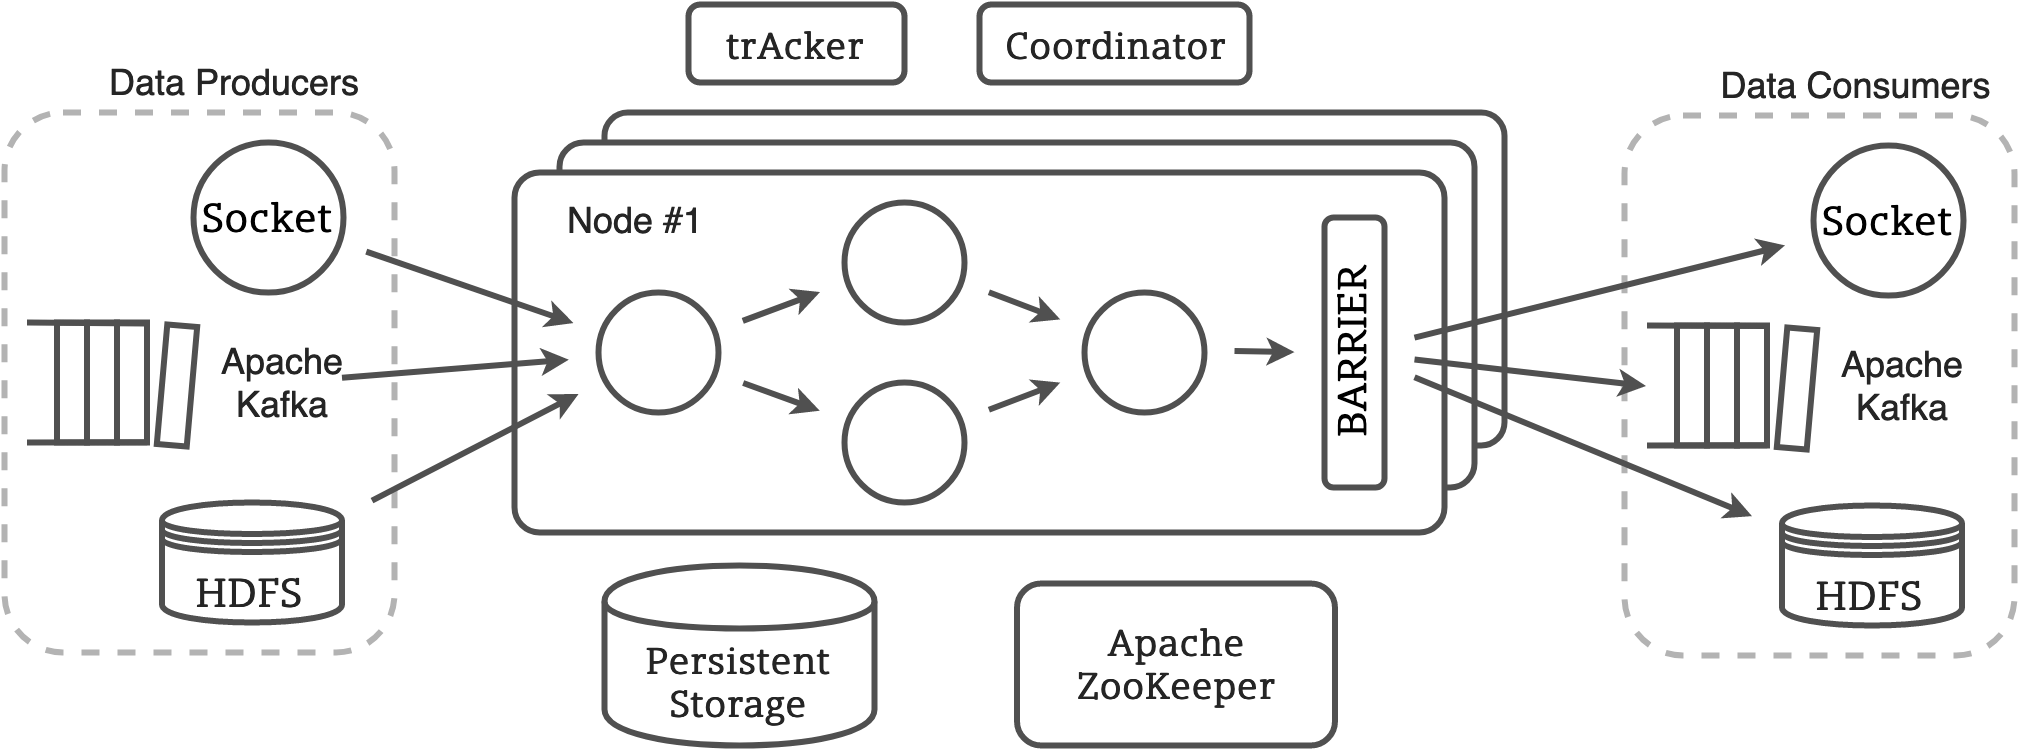
\includegraphics[scale=0.78]{pics/arch}
  \caption{The overview of \FlameStream\ architecture}
  \label {arch}
\end{figure*}

{\bf Node} runs a process called {\it worker}. Worker executes user-defined operations. The computational load is balanced through the distribution of data items among workers. A worker for a data item is determined by the value of a hash function of item payload. Such hash functions can be defined by a user before each logical operation. Each worker can be responsible for one or many ranges of values of hash functions called {\it hash units}. The number of hash-units per worker is a user-defined parameter, and it must be set before the start of computations. 

{\bf Execution graph} is an Akka-based representation of a user-defined logical graph. Execution graph is run by each worker. A data item can be sent to another worker before each operation due to balancing technique and the distribution of hash units. The communication within a node is done via messaging or direct function calls depending on runtime heuristics. A delivery that crosses node boundaries is performed by means of TCP.

{\bf Barrier} is located at the end of each execution graph instance. The barrier has two main responsibilities:

\begin{itemize}
    \item Filtering out possible duplicates or invalid results
    \item Taking a snapshot of the last released element, that is an essential part of providing exactly-once semantics
\end{itemize}

{\bf Acker} is an agent that tracks the processing progress of the system. Acker has two main roles as well. It broadcasts information about input elements nullification that is needed for barrier flushing and coordinates state snapshotting and recovery protocols described in the following sections.

{\bf Apache ZooKeeper} is used as a {\it cluster state manager}. It contains basic system parameters and locations of workers and acker. The usage of ZooKeeper mitigates the need for the dedicated master node.

{\bf Persistent storage} is needed for reliable storing of state snapshot. In case of failures, state snapshot is recovered from the persistent storage. It can be a distributed file system or database (e.g., HDFS, S3, MongoDB, GFS, HBase, etc.).

\subsection{Meta-information structure}

In~\FlameStream\ the meta-information is a tuple of a {\it global time}, a {\it trace}, {\it child ids} and a {\it tombstone flag}.

\[Meta := (GlobalTime, ChildIds[\:], Trace, IsTombstone)\]

Global time is assigned to each input data item $a$ when it enters the system. It is a logical time and identifier of data producer. The identifier of data producer is needed to prevent collisions. Global time of a derivative item is a maximal global time among input elements that affect it. This property is preserved in grouping operation and guarantees that if a data flow element $x$ has global time $GT$ and an input element that is defined by global time $GT$ has been already nullified, then all input elements that affect $x$ have been nullified as well. It allows the system to use global time as an indicator of $Cl^{-1}(D)$. It is worth to note that we do not rely on any clock synchronization between nodes. The only implication of the clock skew is the system degradation regarding latency: 1 ms of the fronts clock difference appends 1 ms to minimal latency.

Map operation is able to generate multiple items from one, and {\em child ids} define an order on them. {\it ChildIds} is an array of child ids, that corresponds to all visited map operations.

If tombstones have been generated, multiple items with the same global time and child ids can exist in the stream. To differentiate them without the comparison of a payload, there is a {\it Trace} value stored in the meta-information. The trace is a xor of all physical operations' ids (random 64-bit identifier) visited by item so far. Invalid item and the corresponding tombstone go along the same path because they have the same payload and the balancing functions are deterministic. Therefore, item and the corresponding tombstone can be revealed via trace matching. 

Therefore, on the one hand, meta-information defines a total order on data flow elements (meta is compared lexicographically). On the other hand, it provides additional information about $Cl^{-1}(D)$ and tombstones.

\subsection{Nullification tracking and barrier flushing}

% In drifting state model, it is assumed that there is a mechanism that periodically provides monotonic, in terms of meta-information, reports about which elements have been nullified. 

As it was mentioned above, in order to implement barrier flushing and state snapshotting mechanisms, there is a need for a mechanism that identifies nullified input elements. The well-known solution for detecting nullified elements is to inject in execution graph special elements that go through the same network channels as ordinary data items and push through data flow elements. When such element is released from the very last node of the execution graph, it means that all previous input elements have been nullified due to FIFO network channels. Flink checkpointing technique is based on this approach~\cite{Carbone:2017:SMA:3137765.3137777}. While it works well in systems that support only acyclic execution graphs, it is unclear how to handle such pushing elements in drifting state cycles. 

To solve the problem we adopt an idea from Apache Storm~\cite{apache:storm}. Storm uses a special agent called {\em Acker} for elements tracking. On each input item, an operation sends to the Acker checksum hash of the corresponding output item and then checksum hash of the input item. Acker XORs all checksums and when the result becomes zero, it means that all items were processed. In this approach, collisions are possible, but they are very unlikely in practice. In our modification, checksum hash is sent together with element global time. This message is called {\it ack}. Acker groups acks by a global time into the structure called {\it ack table}. Once acker receives an ack message with global time {\it GT} and {\it XOR} it updates {\it GT} entry in the table by xoring {\it XOR} with the current value. When an item is sent and later received by the next operation, xoring corresponding {\it XOR}s would yield zero.

Acks are overlapped to make table's entry equal to zero only when an item arrives at the barrier, i.e., ack for receive is sent only after both transformation is done and the ack for the transformed item is sent, as illustrated in Figure~\ref{acker}. In this example, different shapes of items mean different payloads. The ack for the sending of the triangular element is sent before the rectangular one. We expect the channel between the acker and each operation to be FIFO, so ack for the triangular item would be xored before the rectangular. So the two equal values are separated by a distinct one. This technique guarantees that the {\it XOR} for some global time is equal to zero only if there are no in-flight elements with such global time.

\begin{figure}[htbp]
  \centering
  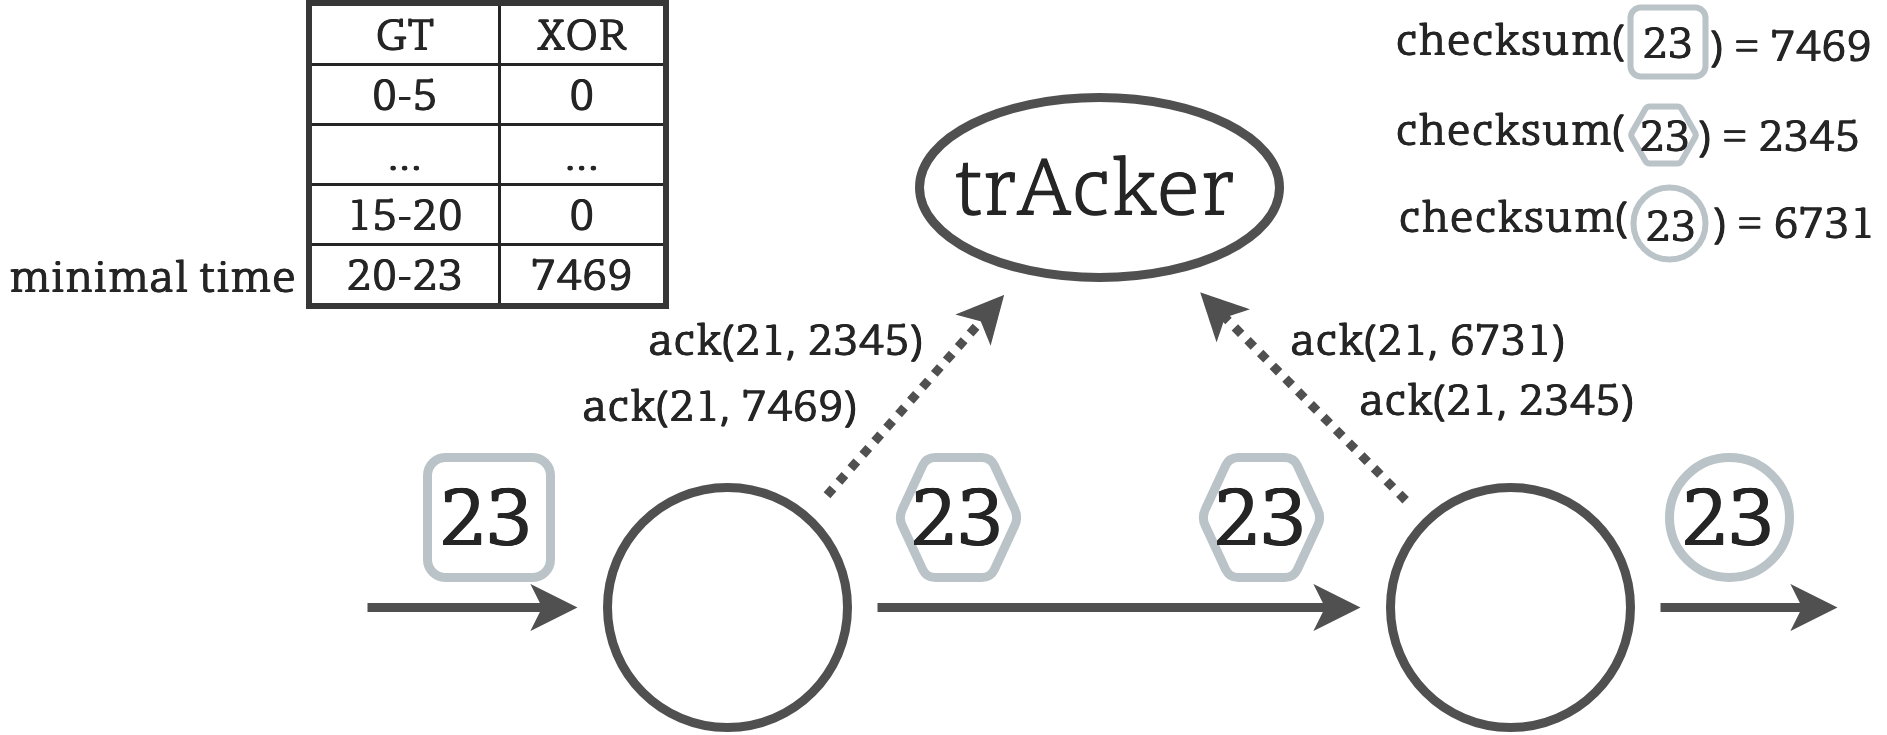
\includegraphics[scale=0.58]{pics/acker}
  \caption{The example of tracking minimal time using acker}
  \label {acker}
\end{figure}

The {\em minimal time} within a stream is the minimal global time with non-zero {\it XOR}. On minimal time changes, acker broadcasts new minimal time to the barrier and operations. An important property of these notifications is monotonicity in terms of global time. Minimal time notifications guarantee that there are no elements in a data flow, except in the barrier, with the given global time and less. It implies that there are tombstones with such global time and less as well. The barrier can release elements with global time {\it GT} once it received notification from acker that the minimal time within the stream is greater than {\it GT} because it means that input element identified by {\it GT} is ready for safe nullification. 

It must be noted that acker can play the role of a worker's coordinator because it observes the progress of the whole system. This property is used further in the implementation of mechanisms for fault tolerance. 

\subsection{Last output element snapshotting}

As we demonstrated in section~\ref{fs-formalism} if consistent state snapshotting is extended by the snapshotting of the last output element, then a system is able to provide exactly once without synchronization between state snapshotting and output elements releasing. 

Minimal time notifications are sent by the acker with monotonically increasing global times. Barrier receives these notifications and releases output items with monotonically increasing global times as well. Hence, the barrier can filter out any items with a global time less than or equal to the global time of the last released item $GT_{last}$ in order to preserve exactly once. To implement this mechanism, there is a need to atomically output items and update $GT_{last}$. To solve this problem, we require the following output protocol with data consumer: 

\begin{itemize}
    \item When minimal time notification is received, barrier send output bundle to the data consumer. This bundle contains all corresponding output items and $GT_{last}$. The consumer must acknowledge that it received the bundle
    \item Barrier does not send new output bundle until the previous one is not acknowledged
    \item Consumer must return last received bundle on barrier's request 
\end{itemize}

This protocol guarantees that $GT_{last}$ and released items are always consistent with each other. It implies that barrier can request the last released bundle and fetch $GT_{last}$ after recovery to avoid duplicates and preserve exactly-once semantics.

Thus, on the one hand, we delegate the part of the basic functionality to data consumers. On the other hand, the requirement on data consumer is not so strong and can be naturally satisfied by real-world consumers (HDFS, Kafka, databases, etc.). 

% \subsection{Input replay}

\subsection{State snapshotting and input replay}

Input replay functionality is commonly used to restore computational process after a failure in stream processing systems~\cite{Carbone:2017:SMA:3137765.3137777, Akidau:2013:MFS:2536222.2536229, apache:storm}. The key idea here is that in case of failure, previously released input data can be retrieved again. Usually, replay is started not from the beginning, but from a certain point. Like other stream processing solutions, our system requires from producers an ability to replay input data. The only difference is that the initial point of replay is defined in terms of global time. Practically, the role of global times can be played by any monotonically increasing sequence, e.g., offsets in Apache Kafka~\cite{kreps2011kafka} or the values of a logical clock. Therefore, this requirement is not a strong limitation for real-life deployments.

In order to inform data producers that some input data will never be used further, a system must take state snapshots. Because of the fact that in~\FlameStream\ there is no need for synchronization between state snapshotting and elements releasing mechanisms, the global time for taking snapshot can be periodically chosen. It is convenient to piggyback on minimal time notifications for triggering state saving. Let $GT_{min}$ be the last received minimal time within the stream. Grouping's buckets in practice are lists sorted by global time. Because of the guarantees provided by minimal time notifications, these lists cannot be modified at any position before the item that corresponds to $GT_{min}$, the immutable prefix and mutable suffix of grouping bucket are shown at Figure~\ref{immutable}. At the same time, because of the grouping semantics, state that is reached after consuming all data items with global times in range $[0..GT_{min})$ is just a window-sized sublist that is located in the immutable part of the bucket, the example is shown in figure~\ref{substate}. Thereby, state snapshotting of different operations can be done asynchronously with each other and with the computational process of the current operation. 

\begin{figure}[htbp]
  \centering
  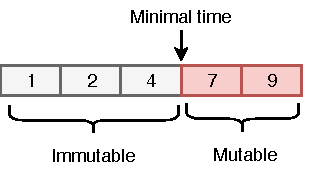
\includegraphics[width=.3\textwidth]{pics/immutable}
  \caption{Grouping bucket won't be modified up to element that corresponds to current minimal time}
  \label {immutable}
\end{figure}

\begin{figure}[htbp]
  \centering
  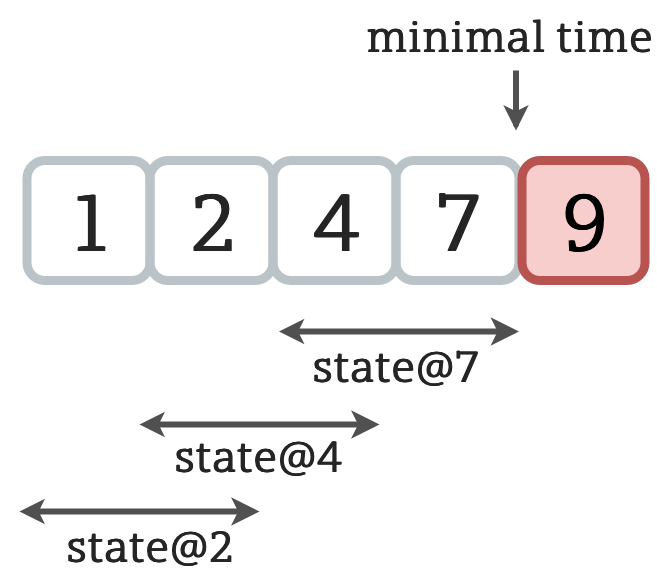
\includegraphics[width=.3\textwidth]{pics/substate}
  \caption{Grouping buckets with window = 2. Window-sized sublists are grouping states at past global times}
  \label {substate}
\end{figure}

Considering the properties mentioned above, the protocol of state snapshotting is the following:

\begin{itemize}
    \item On minimal time event, acker sends a request for the new snapshot along with minimal time notification
    \item When grouping operation receives the request, it asynchronously saves the state and sends back the acceptance message. The local state can be cleared after saving
    \item When barrier receives the request, it waits until producer acknowledges all in-flight bundles, and then sends back the acceptance message to the acker
    \item When acker receives all acceptance messages, it saves the global time of the snapshot to cluster state manager (ZooKeeper) 
\end{itemize}

This protocol is a variation of 2PC and is shown in Algorithm~\ref{state-snapshoting}.

\begin{algorithm}
\caption{State Snapshotting}
\label{state-snapshoting}
  \begin{algorithmic}
    \Process {Acker}
      \State $vertices \gets$ all physical groupings and barrier instances
      \State $snapshotted \gets \varnothing$
      \State $ongoingSnapshot \gets nil$
      \State
      \Event{$\langle MinTime, t \rangle$}
        \If {$ongoingSnapshot = nil$} \Comment{There is no unfinished snapshot}
          \For{{\bf all $v$} $\in vertices$}
            \State \Call{Send}{$v, \langle MinTime_{snap}, t\rangle$}
          \EndFor
          \State $ongoingSnapshot \gets t$
        \EndIf
      \EndEvent
      \Event{$\langle Snapshotted, v\rangle$}
        \State $snapshotted \gets snapshotted \cup v$
        \If {$snapshotted = vertices$}
          \State \Call{Save}{$ongoingSnapshot$} \Comment{Save time to cluster state manager}
          \State $snapshotted \gets \varnothing$
          \State $ongoingSnapshot = nil$
        \EndIf
      \EndEvent
    \EndProcess

    \Process {Grouping}
      \State $bucket[]$ \Comment{List of data items ordered by time}
      \State
      \Event{$\langle MinTime_{snap}, t\rangle$}
        \State \Call{Save}{t, bucket[0, t]} \Comment{Save substate to persistent storage}
        \State \Call{ClearRange}{bucket, 0, t}
        \State \Call{Send}{$acker, \langle Snapshotted, self\rangle$}
      \EndEvent
    \EndProcess

    \Process {Barrier}
      \State $lastAcknowledgedTime \gets -\infty$ \Comment{Time of the last acknowledged bundle by consumer}
      \State $postponedSnapshotTime \gets \infty$
      \State
      \Event{$\langle MinTime_{snap}, t\rangle$}
        \If{$lastAcknowledgedTime \geq t$}
          \State \Call{Send}{$acker, \langle Snapshotted, self\rangle$}
        \Else
          \State $postponedSnapshotTime \gets t$
        \EndIf
      \EndEvent
      \Event{$\langle Ack, t\rangle$}
        \State $lastAcknowledgedTime \gets t$
        \If {$postponedSnapshotTime < lastAcknowledgedTime$}
          \State \Call{Send}{$acker, \langle Snapshotted, self\rangle$}
          \State $postponedSnapshotTime \gets \infty$
        \EndIf
      \EndEvent
    \EndProcess
  \end{algorithmic}
\end{algorithm}

Acker can send requests for the new snapshot not for each minimal time event, e.g., it can skip request if the elapsed time since the last snapshot is less than some threshold. Parameters that influence the frequency of snapshots are in user's scope.

It is worth to note that any persistent key-value storage can be used as a storage for the state. Hash unit of the corresponding grouping operation concatenated with received minimal time can be used as a key. Waiting until barrier sends out all in-flight bundles is the only dependency between state snapshotting and barrier flushing mechanisms, that does not practically influence end-to-end processing latency. 

This protocol satisfies the following properties regarding the global time $GT$ that is written to cluster state manager:
\begin{enumerate}
    \item All stateful operations can restore the state that is reached after consuming all data items with global times in range $[0..GT)$ 
    \item All bundles that contain items with global times in range $[0..GT)$ have been already acknowledged by data consumer 
\end{enumerate}

Hence, this global time can be used as a resuming point after recovery without loss of consistency.

It is worth to note that the proposed protocol is similar to the state snapshotting protocol used in Flink~\cite{Carbone:2017:SMA:3137765.3137777}. The key difference is that in our method, output releasing agents (barriers) do not take part in a distributed transaction (variation of 2PC), due to drifting state model properties shown in section~\ref{fs-model-section}. This difference determines the significant latency decrease that is demonstrated further.

\subsection{Failure detection and recovery}

Typically, distributed systems take into consideration the following types of failures:
\begin{itemize}
    \item Packet loss
    \item Node failure
    \item Network partitioning
\end{itemize}

Network partitioning is the special case of failure because in this case computations cannot be restarted. We believe that in this case, stream processing does not make sense. To the best of our knowledge, there are no open-source stream processing systems that tolerate network partitioning.

As it was described above, acker traces data items using the table of XORs grouped by global time. Therefore, packet loss can be determined by the acker because the corresponding value in acker's table will not be nullified. Node failure can also be observed by the acker through periodical heartbeats. 

In case of packet loss or node failure, acker restarts the computations from the last successful checkpoint. The failure of the acker itself can be detected by the cluster state manager, that triggers the same restart protocol. Restart protocol includes the following steps:

\begin{itemize}
    \item Acker reads the global time of the last snapshot from cluster state manager. After that, it broadcasts this global time to all grouping operations
    \item Grouping operations fetch their states from state storage using the corresponding hash unit and received global time as a key. After that, grouping operations send an acknowledgment that they are ready for processing to the acker 
    \item Barriers request the last released bundle from data consumers and send acknowledgments that they are ready for processing to the acker
    \item When acker receives all acknowledgments from groupings and barriers, it requests data producer to replay starting from the global time of the last snapshot  
\end{itemize}

Proposed protocol guarantees the following properties that allows preserving exactly once:

\begin{itemize}
    \item Processing does not restart until all grouping operations obtain consistent states. The consistency of these states is guaranteed by the state snapshotting protocol
    \item Duplicates are not produced because, at the moment when processing is restarted, it is ensured that barrier has obtained the last released global time and is able to filter out extra items
    \item The last released global time cannot be less than the global time of the last snapshot. Therefore, data cannot be lost. This property is guaranteed in conjunction with the state snapshotting protocol
\end{itemize}

% \subsection{Tracking nullification}

% % As it was defined previously, in our model, only the grouping operation maintains a state and the state depends on the order of incoming items. Therefore, to achieve deterministic processing, there is a need to enforce the right order. However, conservative methods for the order enforcing are based on buffering~\cite{Li:2008:OPN:1453856.1453890} and can imply high latency overhead. The main difficulty here is that items can be easily reordered within stream processing systems because of asynchrony and the possible existence of multiple paths between two nodes. 

% % In~\cite{hiddenSeim} an optimistic approach to handle out-of-order items was introduced. The key idea behind it is that grouping can produce invalid results, but they must be filtered out at the barrier. Therefore, there is a need to buffer output items at the barrier before it is ensured that there are no invalid in-flight items and they cannot be generated. It is convenient to release items by global times.

% To track the global time of in-flight items we adopt an idea of {\it acker task} inspired by Apache Storm~\cite{apache:storm}. Acker tracks data items using a checksum hash. When the item is sent or received by an operation, its global time and checksum are sent to the acker. This message is called {\it ack}. Acker groups acks by a global time into the structure called {\it ack table}. Once acker receives an ack message with global time {\it GT} and {\it XOR} it updates {\it GT} entry in the table by xoring {\it XOR} with the current value. When an item is sent and later received by the next operation, xoring corresponding {\it XOR}s would yield zero.

% Acks are overlapped to nullify table's entry only when an item arrives at the barrier. That is, ack for receive is sent only after both processing and the ack sending for the transformed item, as illustrated in Figure~\ref{acker}. Different shapes of items mean different payloads. The ack for the sending of the triangular element is sent before the rectangular one. We expect the channel between the acker and each operation to be FIFO, so ack for the triangular item would be xored before the rectangular. So the two equal values are separated by distinct one. This technique guarantees that the {\it XOR} for some global time is equal to zero only if there are no in-flight elements with such global time.

% \begin{figure}[htbp]
%   \centering
%   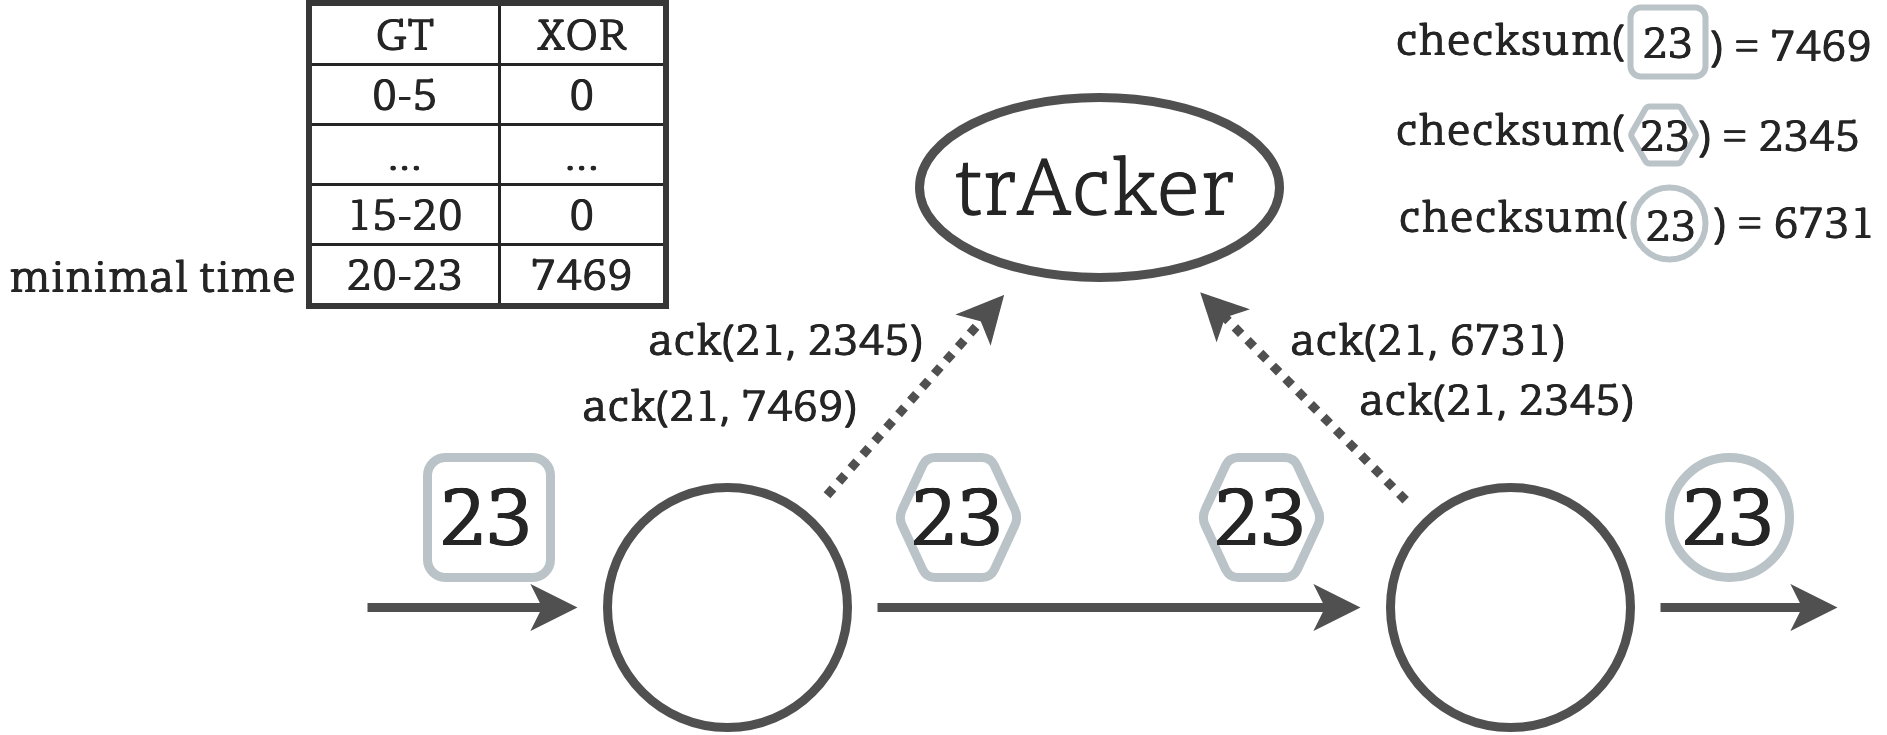
\includegraphics[scale=0.58]{pics/acker}
%   \caption{The example of tracking minimal time using acker}
%   \label {acker}
% \end{figure}

% The minimal time within a stream is the minimal global time with non-zero {\it XOR}. On minimal time changes, acker broadcasts new minimal time to the barrier and operations. Minimal time notifications plays the same role as {\em low-watermarks} in OOP architecture~\cite{Li:2008:OPN:1453856.1453890}. Therefore, the barrier can release elements with global time {\it GT} once it received notification from acker that the minimal time within the stream is greater than {\it GT}.

% The important implication of ack-table structure is that items that was generated by a single input event become ready for release at the same moment.

% To ensure that no fronts can generate item with the specific timestamp, each front periodically sends to acker special message called {\it report}, which promises that front will not generate items with a timestamp lower than the reported. The value in the ack table can become zero only after the corresponding report arrives.

% It must be noted that acker can play the role of worker's coordinator because it observes the progress of the whole system. This property is used further in the implementation of mechanisms for fault tolerance. 

% \subsection{System architecture}

% \FlameStream\ is implemented in Java, using Akka framework for messaging. An overview of the \FlameStream\ system model and architecture is shown in Figure~\ref{arch}. The main componets are:

% {\bf Acker} supervises computation process and play role of coordinator in consistency protocols described in following sections.

% {\bf Graph} is deployed on each node and process a partition of data that corresponds to its hash range. The communication within a node is done via messaging or direct function calls depending on runtime heuristics, a delivery that crosses node boundaries is performed by means of TCP.

% {\bf Barrier} is located at the end of each graph instance. It filters duplicates and invalid data and delivers it to data consumers.

% {\bf Data producers and data consumers} are deployed separately and communicate with system via defined protocols

% {\bf Apache ZooKeeper} is used as a {\it cluster state manager}. The usage of ZooKeeper mitigates the need for the dedicated master node.

% {\bf Persistent storage} is needed for reliable state saving to mitigate failures, in can be a distributed filesystem or database (e.g., HDFS, S3, MongoDB, GFS, HBase, ...)


% \begin{figure*}[htbp]
%   \centering
%   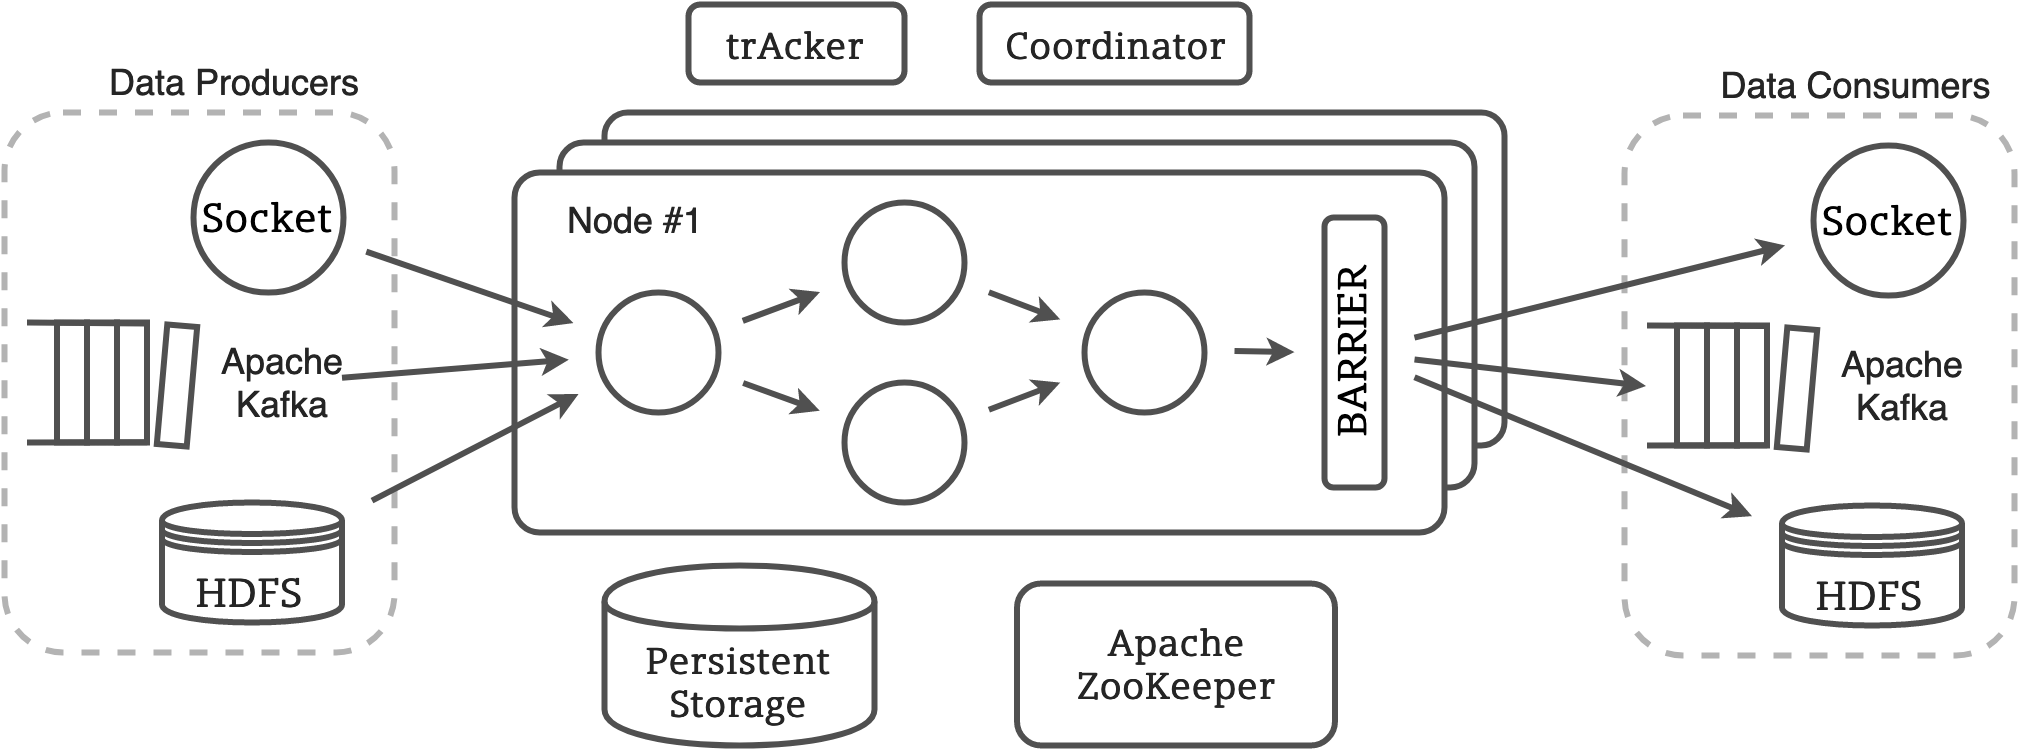
\includegraphics[scale=0.78]{pics/arch}
%   \caption{The overview of \FlameStream\ physical architecture}
%   \label {arch}
% \end{figure*}

% % In this section, we describe how consistency guarantees can be provided within the proposed model in case of failures. We define three mechanisms which are necessary both for consistent processing and for fast and reliable recovery: {\em input replay}, {\em barrier flushing}, and {\em state snapshotting}. Input replay is used in case of failures for computations restoring. Barrier flushing is responsible for filtering out of the extra items. State snapshotting allows replaying input stream from certain points, eliminating the need for storing the full input data. We demonstrate how these mechanisms behave in recovery processes and why consistency semantics is preserved.

% % It is worth to mention that we rely strongly on the properties of the proposed model and its implementation. Firstly, we expect that processing is deterministic, i.e., several independent runs with the same input data produce exactly the same result. This property is guaranteed by the fact that all supported operations produce deterministic results. Secondly, we suppose that there is an agent that can coordinate protocols for fault tolerance. The role of such coordinator is played by the acker. Thirdly, we use the fact that acker broadcasts minimal time notifications when it is guaranteed that there are no in-flight data items with particular global time and such items cannot be generated further. Additionally, we exploit the simple structure of the grouping's state, which is a list sorted by global time. These features allow us to build efficient techniques for barrier flushing and operations' state management, which preserve exactly-once semantics and almost do not depend on each other.

% % It is important to notice that at most once semantics is preserved even in case of failures without any additional logic. Such behavior is achieved because we assume that data producers do not replay input data if it is not requested and within our system, data can only be lost, but not duplicated. Therefore, we mainly focus on providing at least once and exactly-once semantics.

% \subsection{Input replay}
% Input replay functionality is commonly used to restore computational process after a failure in stream processing systems~\cite{Carbone:2017:SMA:3137765.3137777, Akidau:2013:MFS:2536222.2536229, apache:storm}. The key idea here is that in case of failure, previously released input data can be retrieved again. Usually, replay is started not from the beginning, but from a certain point. Like other stream processing solutions, our system requires from producers an ability to replay input data. The only difference is that the initial point of replay is defined in terms of the global time. Practically, the role of global times can be played by any monotonically increasing sequence, e.g., offsets in Apache Kafka~\cite{kreps2011kafka} or the values of a logical clock. Therefore, this requirement is not a strong limitation for real-life deployments.

% \subsection{Barrier flushing}
% Minimal time notifications are sent by the acker with monotonically increasing global times. Barrier receives these notifications and releases output items with monotonically increasing global times as well. Hence, the barrier can process data in idempotent fashion simply by filtering out any items with a global time less than or equal to the global time of the last released item $GT_{last}$. 

% Therefore, the barrier has a state - $GT_{last}$, and this state is applied for avoiding duplicates in case of failure and subsequent input replay. Exactly-once semantics is possible only if there are no inconsistencies between released items and $GT_{last}$, so there is a need to atomically output items and update $GT_{last}$. To solve this problem, we require the following output protocol with data consumer: 

% \begin{itemize}
%     \item When minimal time notification is received, barrier send output bundle to the data consumer. This bundle contains all corresponding output items and $GT_{last}$. The consumer must acknowledge that it received the bundle
%     \item Barrier does not send new output bundle until the previous one is not acknowledged
%     \item Consumer must return last received bundle on barrier's request 
% \end{itemize}

% This protocol guarantees that $GT_{last}$ and released items are always consistent with each other. It implies that barrier can request the last released bundle and fetch $GT_{last}$ after recovery to avoid duplicates and preserve exactly-once semantics. It should be noted that for at least once semantics, contract with the consumer can be relaxed: it is not required to store the last received bundle.

% \subsection{State snapshotting}
% In case of failures, a producer can replay all previously sent data items on recovery without loss of exactly-once semantics. Such behavior is achieved because processing results are deterministic and all possible duplicates are filtered out at the barrier. However, this approach can be memory and time demanding. 

% Therefore, there is a need to take a snapshot of operations' state periodically and to replay on recovery from a certain point that corresponds to the previous snapshot. Global time is the most natural indicator of such points within our model because the grouping's state can be easily reverted to the specified global time and the data producer supports replay in terms of global time.   

% Hence, the global time for taking snapshot must be periodically chosen. It is convenient to piggyback on minimal time notifications for triggering state saving. Let $GT_{min}$ be the last received minimal time within the stream. Grouping's buckets in practice are lists sorted by global time. Because of the guarantees provided by minimal time notifications, these lists cannot be modified at any position before the item that corresponds to $GT_{min}$, the immutable prefix and mutable suffix of grouping bucket are shown at Figure~\ref{immutable}. At the same time, because of the grouping semantics, state that is reached after consuming all data items with global times in range $[0..GT_{min})$ is just a window-sized sublist that is located in the immutable part of the bucket, the example is shown in figure~\ref{substate}. Thereby, state snapshotting of different operations can be done asynchronously with each other and with the computational process of the current operation. 

% \begin{figure}[htbp]
%   \centering
%   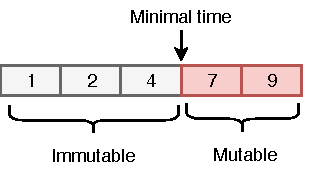
\includegraphics[width=.3\textwidth]{pics/immutable}
%   \caption{Grouping bucket won't be modified up to element that corresponds to current minimal time}
%   \label {immutable}
% \end{figure}

% \begin{figure}[htbp]
%   \centering
%   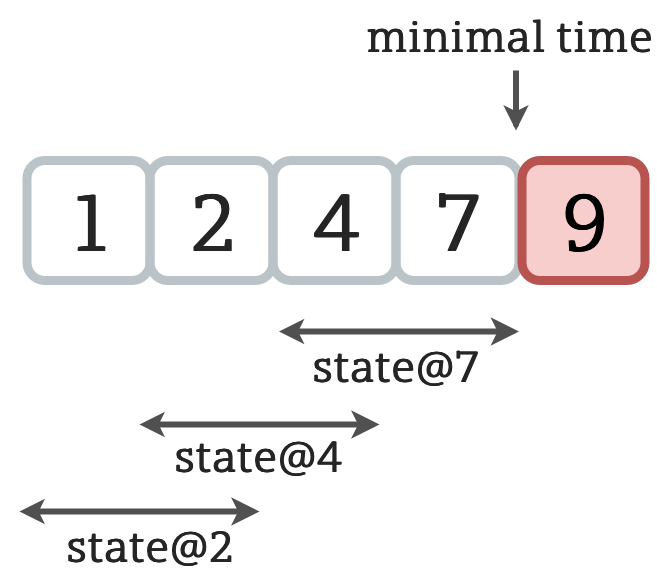
\includegraphics[width=.3\textwidth]{pics/substate}
%   \caption{Grouping buckets with window = 2. Window-sized sublists are grouping states at past global times}
%   \label {substate}
% \end{figure}

% Considering the properties mentioned above, the protocol of state snapshotting is the following:

% \begin{itemize}
%     \item On minimal time event, acker sends a request for the new snapshot along with minimal time notification
%     \item When grouping operation receives the request, it asynchronously saves the state and sends back the acceptance message. The local state can be cleared after saving
%     \item When barrier receives the request, it waits until producer acknowledges all in-flight bundles, and then sends back the acceptance message to the acker
%     \item When acker receives all acceptance messages, it saves the global time of the snapshot to cluster state manager (ZooKeeper) 
% \end{itemize}

% This protocol is shown in Algorithm~\ref{state-snapshoting}.

% \begin{algorithm}
% \caption{State Snapshotting}
% \label{state-snapshoting}
%   \begin{algorithmic}
%     \Process {Acker}
%       \State $vertices \gets$ all physical groupings and barrier instances
%       \State $snapshotted \gets \varnothing$
%       \State $ongoingSnapshot \gets nil$
%       \State
%       \Event{$\langle MinTime, t \rangle$}
%         \If {$ongoingSnapshot = nil$} \Comment{There is no unfinished snapshot}
%           \For{{\bf all $v$} $\in vertices$}
%             \State \Call{Send}{$v, \langle MinTime_{snap}, t\rangle$}
%           \EndFor
%           \State $ongoingSnapshot \gets t$
%         \EndIf
%       \EndEvent
%       \Event{$\langle Snapshotted, v\rangle$}
%         \State $snapshotted \gets snapshotted \cup v$
%         \If {$snapshotted = vertices$}
%           \State \Call{Save}{$ongoingSnapshot$} \Comment{Save time to cluster state manager}
%           \State $snapshotted \gets \varnothing$
%           \State $ongoingSnapshot = nil$
%         \EndIf
%       \EndEvent
%     \EndProcess

%     \Process {Grouping}
%       \State $bucket[]$ \Comment{List of data items ordered by time}
%       \State
%       \Event{$\langle MinTime_{snap}, t\rangle$}
%         \State \Call{Save}{t, bucket[0, t]} \Comment{Save substate to persistent storage}
%         \State \Call{ClearRange}{bucket, 0, t}
%         \State \Call{Send}{$acker, \langle Snapshotted, self\rangle$}
%       \EndEvent
%     \EndProcess

%     \Process {Barrier}
%       \State $lastAcknowledgedTime \gets -\infty$ \Comment{Time of the last acknowledged bundle by consumer}
%       \State $postponedSnapshotTime \gets \infty$
%       \State
%       \Event{$\langle MinTime_{snap}, t\rangle$}
%         \If{$lastAcknowledgedTime \geq t$}
%           \State \Call{Send}{$acker, \langle Snapshotted, self\rangle$}
%         \Else
%           \State $postponedSnapshotTime \gets t$
%         \EndIf
%       \EndEvent
%       \Event{$\langle Ack, t\rangle$}
%         \State $lastAcknowledgedTime \gets t$
%         \If {$postponedSnapshotTime < lastAcknowledgedTime$}
%           \State \Call{Send}{$acker, \langle Snapshotted, self\rangle$}
%           \State $postponedSnapshotTime \gets \infty$
%         \EndIf
%       \EndEvent
%     \EndProcess
%   \end{algorithmic}
% \end{algorithm}

% Acker can send requests for the new snapshot not for each minimal time event, e.g., it can skip request if the elapsed time since the last snapshot is less than some threshold. Parameters that influence the frequency of snapshots are in user's scope.

% It is worth to note that any persistent key-value storage can be used as a storage for the state. Hash unit of the corresponding grouping operation concatenated with received minimal time can be used as a key. Waiting until barrier sends out all in-flight bundles is the only dependency between state snapshotting and barrier flushing mechanisms, that does not practically influence end-to-end processing latency. 

% This protocol satisfies the following properties regarding the global time $GT$ that is written to cluster state manager:
% \begin{enumerate}
%     \item All stateful operations can restore the state that is reached after consuming all data items with global times in range $[0..GT)$ 
%     \item All bundles that contain items with global times in range $[0..GT)$ have been already acknowledged by data consumer 
% \end{enumerate}

% Hence, this global time can be used as a resuming point after recovery without loss of consistency.

% \subsection{Failure detection and recovery}
% Typically, distributed systems take into consideration the following types of failures:
% \begin{itemize}
%     \item Packet loss
%     \item Node failure
%     \item Network partitioning
% \end{itemize}

% Network partitioning is the special case of failure because in this case computations cannot be restarted. We believe that in this case, stream processing does not make sense. To the best of our knowledge, there are no open-source stream processing systems that tolerate network partitioning.

% As it was described above, acker traces data items using the table of XORs grouped by global time. Therefore, packet loss can be determined by the acker because the corresponding value in acker's table will not be nullified. Node failure can also be observed by the acker through periodical heartbeats. 

% In case of packet loss or node failure, acker restarts the computations from the last successful checkpoint. The failure of the acker itself can be detected by cluster state manager, that triggers the same restart protocol. Restart protocol includes the following steps:

% \begin{itemize}
%     \item Acker reads the global time of the last snapshot from cluster state manager. After that, it broadcasts this global time to all grouping operations
%     \item Grouping operations fetch their states from state storage using the corresponding hash unit and received global time as a key. After that, grouping operations send an acknowledgment that they are ready for processing to the acker 
%     \item Barriers request the last released bundle from data consumers and send an acknowledgments that they are ready for processing to the acker
%     \item When acker receives all acknowledgments from groupings and barriers, it requests data producer to replay starting from the global time of the last snapshot  
% \end{itemize}

% Proposed protocol guarantees the following properties:

% \begin{itemize}
%     \item Processing does not restart until all grouping operations obtain consistent states. The consistency of these states is guaranteed by the state snapshotting protocol
%     \item Duplicates are not produced because, at the moment when processing is restarted, it is ensured that barrier has obtained the last released global time and is able to filter out extra items
%     \item The last released global time cannot be less than the global time of the last snapshot. Therefore, data cannot be lost. This property is guaranteed in conjunction with the state snapshotting protocol
% \end{itemize}

% Therefore, the proposed protocol can be used for system restart without loss of exactly once semantics. Regarding at least once semantics, all protocol actions are the same, except waiting until the barriers are ready.
